\section{Anlagenbeschreibung}

\begin{figure}[H]
   \centering
   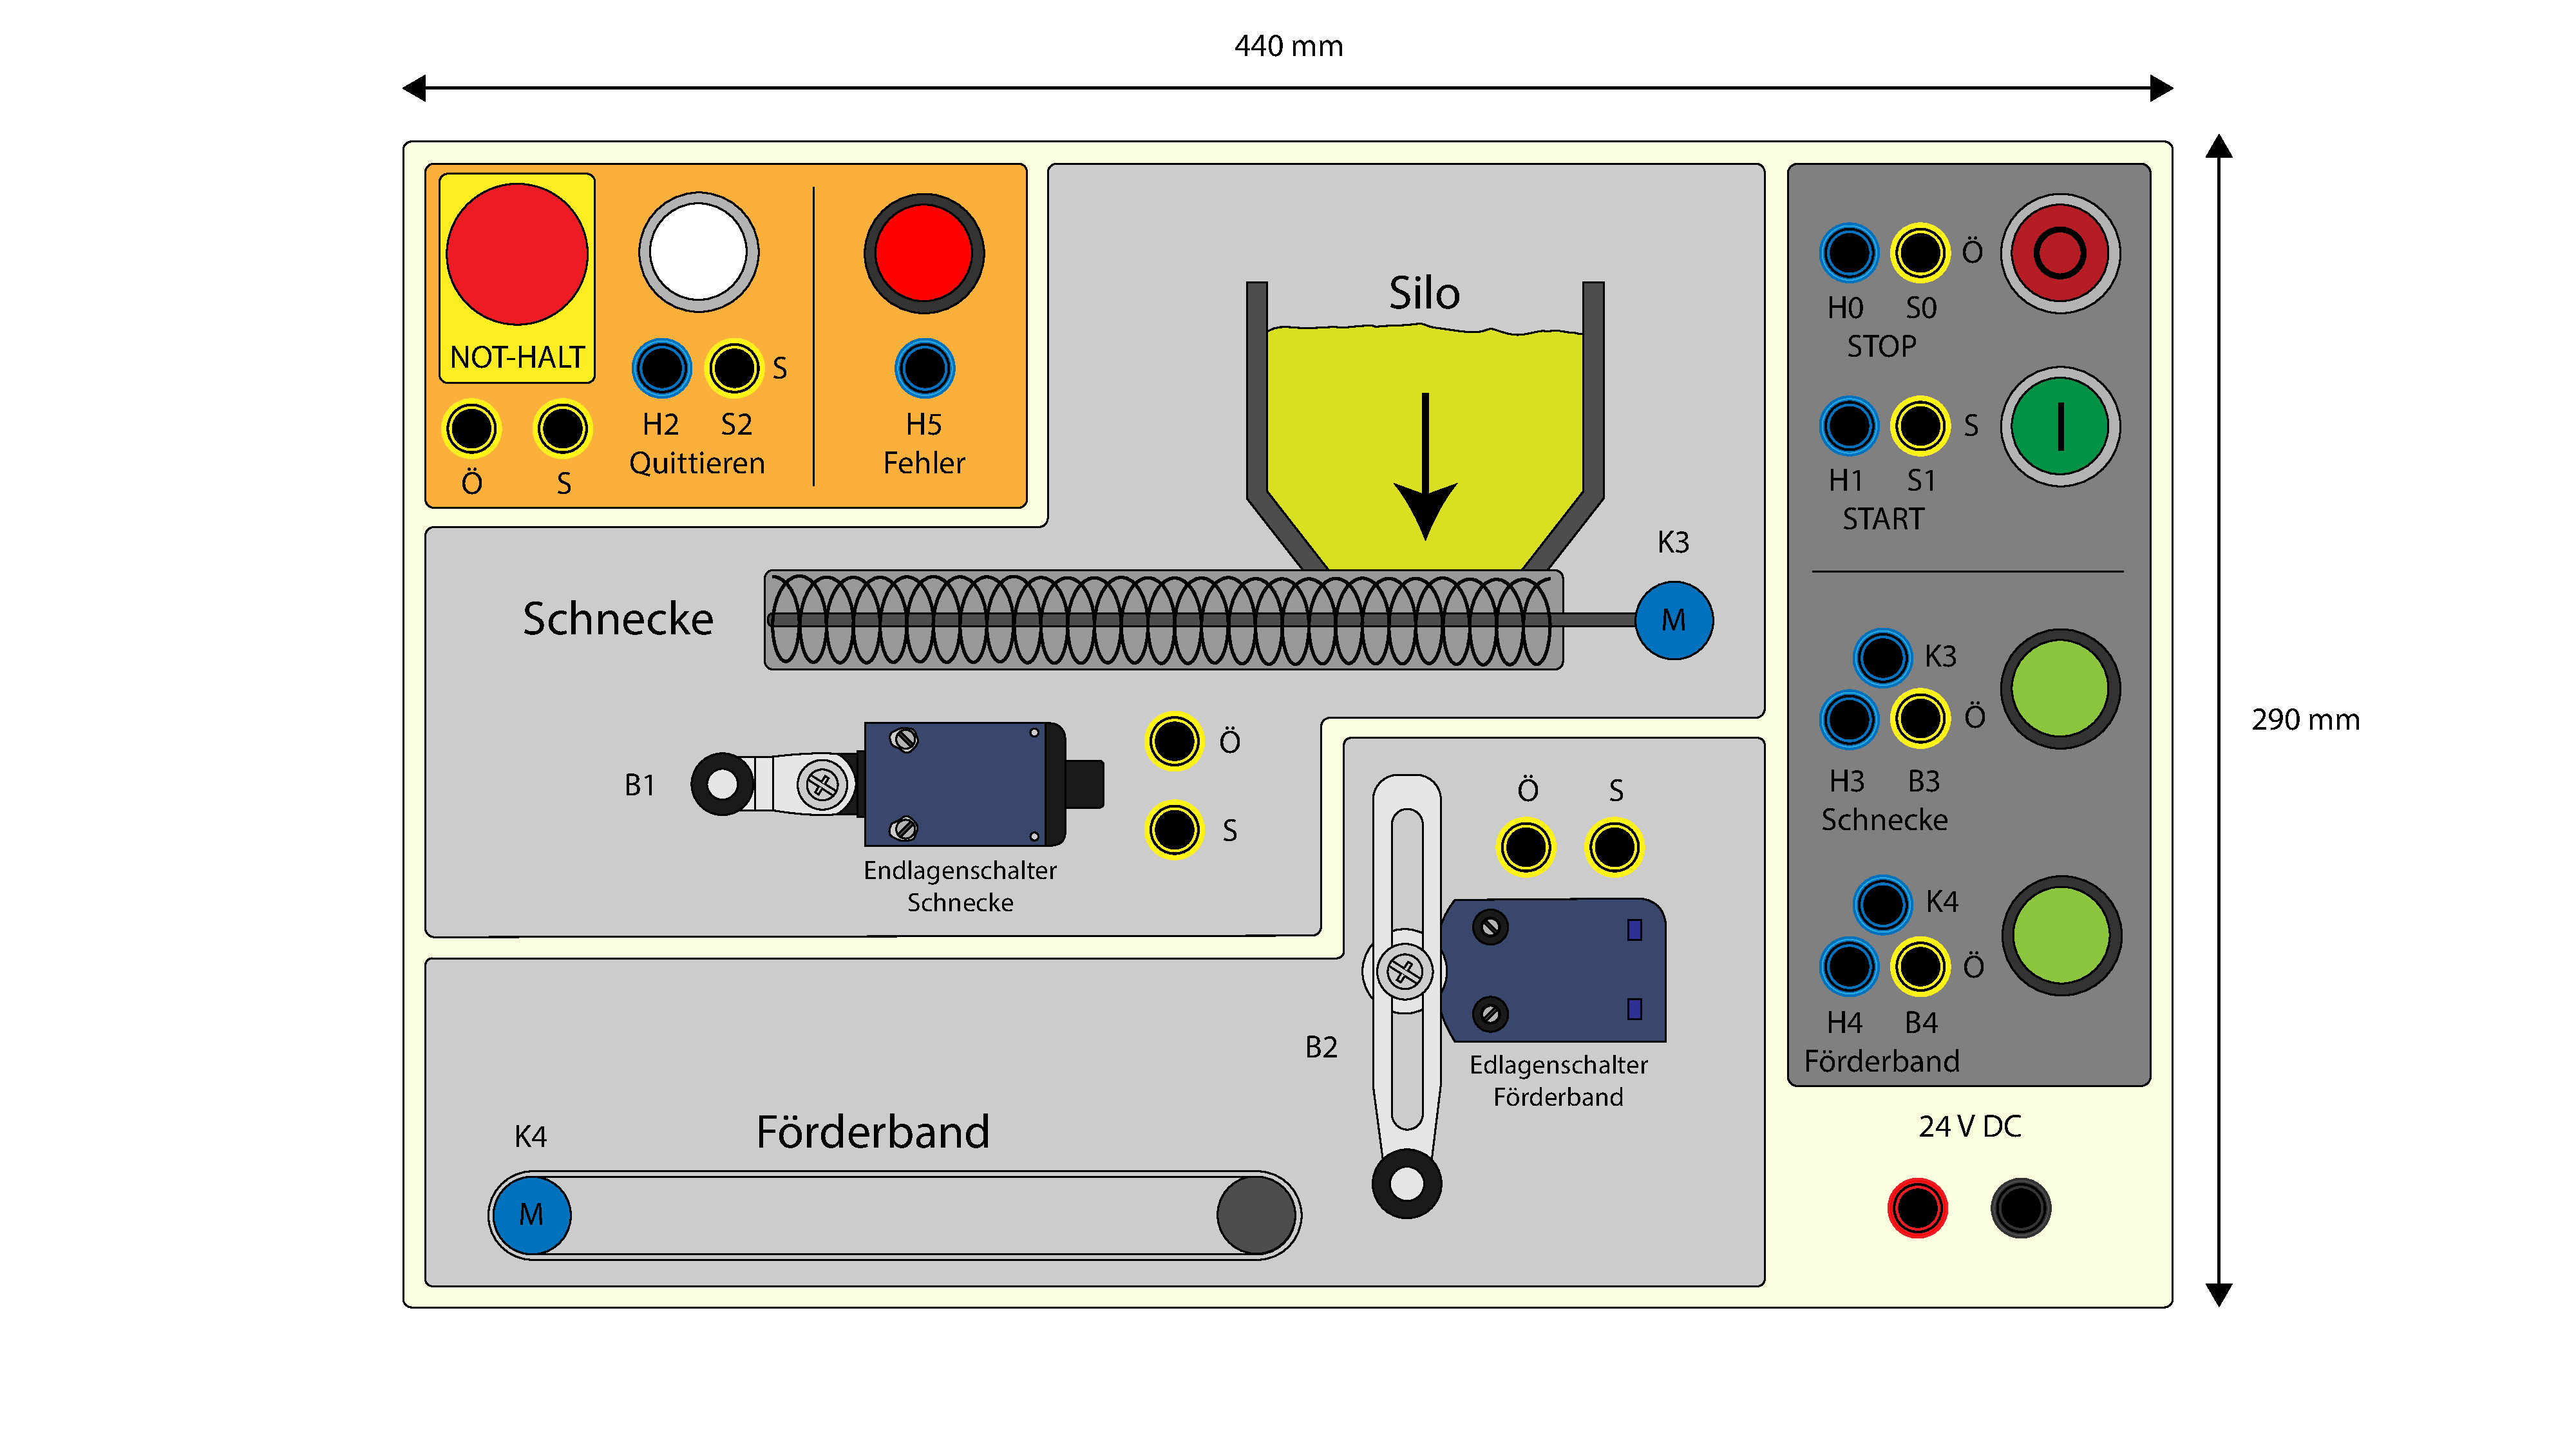
\includegraphics[width=1.0\textwidth]{Bilder/Aufbauplan_Vorderseite.pdf}
   \caption[Technologieschema]{Technologisches Schema der Anlage \glqq Silo mit Förderanlage\grqq{}}
   \label{fig:Bild1}
\end{figure}

Die Versuchsanlage kann sich grundsätzlich in drei Betriebszustände befinden. Dabei handelt es sich um den \textbf{betriebsbereiten Zustand}, den \textbf{Normalbetrieb} und den \textbf{Fehlerfall}. Diese sind nachfolgend beschrieben.

\subsection{Betriebsbereiter Zustand}

Zunächst muss die Stromversorgung hergestellt werden. Der betriebsbereite Zustand wird erreicht, wenn für die Anlage kein Fehler detektiert wird. Zusätzlich dürfen die Endlagen der Förderschnecke und des Förderbandes (B1, B2) nicht auslösen. Die Motoren müssen ausgeschaltet sein, d.h. die SPS erhält FALSE-Signale der Hilfskontakte (B3, B4) der Schütze.\\
Sind die vorangegangenen Bedingungen erfüllt, blinkt der START-Leuchtdrucktaster (H1) mit einer vorgegeben Frequenz von f = 1 Hz. Der STOP-Leuchtdrucktaster (H0) ist ausgeschaltet.

\subsection{Normalbetrieb}

Die Anlage wird durch das Drücken des START-Leuchtdrucktasters (S1) vom betriebsbereiten Zustand in den Normalbetrieb überführt. Der START-Leuchtdrucktaster (H1) hört zu blinken auf und leuchtet nun dauerhaft. Der STOP-Leuchtdrucktaster (H0) leuchtet ebenfalls dauerhaft. Befindet sich die Anlage im Normalbetrieb, soll der Prozess des Materialtransportes von einer Förderschnecke über ein Förderband simuliert werden. Die Ansteuerung der Förderschnecke und des Förderbandes erfolgt jeweils über eine zugeordnete Motorsteuerung. Die modellhaft dargestellten Motoren werden über Hilfsschütze (K3, K4) angesteuert. Der Schaltzustand der Schütze (B3, B4) wird über Hilfskontakte einerseits zur weiteren Auswertung auf die SPS (S7-1500) rückgeführt, andererseits erfolgt die Signalisierung an den Anwender mittels Leuchtmelder (H3, H4). Damit ein fehlerfreier Transport gewährleistet wird, muss das Förderband vier Sekunden vor der Schnecke anlaufen. Ebenfalls ist ein Nachlauf des Förderbandes von fünf Sekunden nach dem Stoppen der Förderschnecke erforderlich. \\
Die Anlage besitzt sowohl für die Förderschnecke als auch das Förderband einen mechanischen Endlagensensor (B1, B2). Das Erreichen der Endlagen wird der SPS signalisiert. \\
Die Anlage wird durch das Drücken des STOP-Leuchtdrucktasters (S0) angehalten.

\subsection{Fehlerfall}

Tritt ein vom Normalbetrieb abweichender Anlagenzustand auf, wird dieser über die Steuerung bzw. das Steuerungsprogramm erkannt und über das Blinken des FEHLER-Leuchtmelders (H5) signalisiert (Blinktakt 1 Hz). Weiterhin findet ein NOT-Halt statt, so dass keine Gefährdung mehr von der Anlage ausgeht. Der Nutzer muss anschließend den Fehler beheben und diesen über einen QUITTIER-Taster (S2) bestätigen. Aus Sicherheitsgründen sollen sowohl kritische als auch unkritische Fehler quittiert werden. Die Anlage befindet sich nun wieder im betriebsbereiten Zustand. Über das erneute Betätigen des START-Leuchtdrucktasters (S1) nimmt die Anlage ihren Normalbetrieb wieder auf. \\
Es ist möglich verschiedene Fehlersituationen an der Anlage zu simulieren. Diese werden folgendermaßen unterteilt:

\begin{enumerate}
    \item Kritische Fehler
    \begin{itemize}
        \item NOT-Halt Betätigung
        \item Unplausible Sensorsignale
        \item Fehlende Rückmeldung der Motorschütze
        \item Mechanische Blockierung der Endlagensensoren
        \item Abweichung innerhalb eines F-Kanals (Ein-/Ausgänge)
    \end{itemize}
    \item Unkritische Fehler
    \begin{itemize}
        \item Überschreiten der SPS-Zykluszeit (Watchdog-Meldung)
        \item Drahtbruch in der Signalleitung des START- oder STOP-Tasters
        \item Ausfall der SPS (Verlust der Spannungsversorgung)
        \item Förderband läuft nach Schnecke an
        \item Förderband stoppt vor Schnecke
    \end{itemize}
\end{enumerate}

Tritt einer der beschriebenen Fehlerfälle auf, wird die Anlage gestoppt. Es muss erst die Fehlerfreiheit vom Nutzer sichergestellt und quittiert werden, um die Anlage erneut zu starten.